\documentclass[11pt,a4paper]{article}
\usepackage{shared-style}
\usepackage{graphicx}
\usepackage{hyperref}
\usepackage{float}
\usepackage{caption}

\shorttitle{Generative AI System for Images}
\shortauthors{Maltoni \& de Mingo Arroyo}

\begin{document}

\papertitle{Generative AI System for Images}
\paperauthors{Adam Maltoni, Ibón de Mingo Arroyo \\[0.3em] \textit{Advisor:} Alberto Suárez González}
\paperdate{May 2025}

\begin{abstract}
The objective of this project is to construct and design an image generation system based on diffusion models to create black-and-white or color images. The main characteristic of the system is its flexibility, as it allows the user to experiment with different parts of the image generation process in a simple and intuitive way.

The module begins with the implementation of three distinct types of diffusion processes for noise injection: Variance Exploding (VE) based on Brownian motion, Variance Preserving (VP) which utilizes Ornstein-Uhlenbeck, and Sub-Variance Preserving (Sub-VP), a variant of VP.

For image generation, we implement various sampling algorithms that transform noise into synthetic images. Among them are the Euler-Maruyama integrator (which is theoretically the simplest), the Predictor-Corrector method, Probability Flow ODE (which has a deterministic approach), and Exponential Integrator. These different sampling techniques allow the user to experiment with the quality, speed, and diversity of the generated images. We also incorporate two types of noise intensity schedules: the linear schedule, which is more direct and predictable, and the cosine schedule, which is smoother and more natural. Understanding the functioning of both schedules helps to improve the final quality of the images.

The system also includes a quantitative metrics module that serves to evaluate the quality of the generated images more objectively. The three implemented metrics are: Bits Per Dimension (BPD), which evaluates the model's understanding of the data; Fréchet Inception Distance (FID), which compares the statistical similarity with real images; and Inception Score (IS), which measures the quality and diversity of the generated images.

Finally, our system is not limited to just generating images. We implement control mechanisms such as class-conditioned sampling (where one can specify which class to generate, e.g., a '3' from the MNIST dataset) and imputation, which allows editing specific parts of an image while keeping the rest intact.

This work represents a complete experimental platform that helps to get started with diffusion models using a simple and practical methodology.

\textbf{Keywords:} Generative AI, diffusion models, conditioning, machine learning, sampling, noise injection, metrics, performance.
\end{abstract}

\tableofcontents
\newpage

\section{Introduction}
The purpose of this project has been to create a generative artificial intelligence system, based on diffusion models, capable of generating color images in a controlled and flexible manner. Our main idea was not only to build a functional model but also to investigate the different variants of the module and observe how the different configurations affect the generated images. For the realization of the module, key concepts of machine learning are used, such as probabilistic modeling, stochastic processes, and score function learning. These theoretical and computational elements are essential to train and guide the model in the image generation process from pure noise towards coherent images.

The implemented module contains five main components for its functionality. The first one includes the three diffusion processes that are used to gradually introduce noise into the data (Variance Exploding, Variance Preserving, and Sub-Variance Preserving). Next are the sampling algorithms used to reverse this process and synthesize images, which are Euler-Maruyama, Predictor-Corrector, Exponential Integrator, and Probability Flow ODE. The module also contains noise schedule programming schemes (Linear and Cosine), the metrics used to evaluate the quality of the images generated by the model (BPD, FID, IS), and, finally, mechanisms that allow generation to be controlled through class conditioning or image completion.

\section{State of the Art}
Synthetic image generation through artificial intelligence is one of the most developed areas within machine learning in recent years. In this project, a generative system capable of producing images in a configurable and controlled way is designed. The developed system relies on a score model based on a U-Net type architecture, which is trained to learn the inverse behavior of the image degradation process into noise. Through this model, and by using different samplers and integrators, it is possible to generate realistic images starting from pure noise. Furthermore, a method to condition generation by class and another for the imputation of missing data in images is included.

Diffusion models have gained a lot of relevance in recent years within the field of generative artificial intelligence. Their operation is based on a two-phase process that transforms an image into noise and then attempts to reconstruct it. This idea is being very effective for generating high-quality images and is the basis of some of the current image generation systems.

The diffusion process starts with an image from our training set to which noise is progressively applied until it turns into pure noise. We call this the forward process. This step does not require learning, since the behavior is determined by a stochastic differential equation that dictates all the steps of the noise injection process into the image.

Learning occurs during the model training, which focuses on the reverse process. In this step, the neural network is trained to estimate the score, that is, the gradient of the log-probability of the data at each instant of noise. To do this, it observes many intermediate samples generated by the forward process and learns to predict in which direction the noise should move to resemble a real image again. The model we have used is based on this idea and employs a U-Net type neural network to estimate the score.

There are different ways to define the evolution of noise in the forward process, which affects not only the model training but also the reverse process and the quality of the generated images. In this project, three main variants have been worked on: VE (Variance Exploding), VP (Variance Preserving), and Sub-VP. Each variant has a different stochastic differential equation to carry out the diffusion process, meaning they have different practical behaviors.

In the case of VE (Variance Exploding), the variance of the noise grows over time, causing the images to degrade faster towards pure noise. This process simulates Brownian motion and does not have a drift term, only a growth in dispersion. On the other hand, in VP (Variance Preserving), noise is added in such a way that the total variance of the sample remains constant throughout the process. As time passes, the image becomes blurrier, but without the noise blowing up. In this project, the VP process is based on an Ornstein-Uhlenbeck type equation, in which both the drift term and the diffusion term depend on time. Finally, Sub-VP (Sub-Variance Preserving) is a variant of VP that modifies the coefficients of the drift term equation (it is more complex since the noise scheme must be integrated), achieving a more progressive transition between image and noise.

On the other hand, when using VP and Sub-VP, it must be considered that they depend on a function that defines the amount of noise added in each step of the forward process. This function is known as the noise schedule. In this work, two options have been implemented: a linear schedule, which adds noise constantly, and a cosine function-based schedule, which adjusts the noise intensity more smoothly and progressively, yielding better results in certain scenarios.

Once the neural network is trained with the score, the reverse process is carried out to reconstruct images from random noise. For this, it is necessary to apply numerical integration methods, known as samplers, which allow simulating the path from pure noise to the reconstruction of an image similar to the samples used during training. Because the reverse diffusion process cannot be solved exactly in most cases since it depends on complex stochastic differential equations, these schemes are used to build approximate trajectories that the model can follow during generation.

In this system, the following options have been implemented: the Euler-Maruyama integrator, the Predictor-Corrector method, Probability Flow ODE, and an Exponential Integrator. Each of these methods yields different results depending on the context and the diffusion process used.

Euler-Maruyama is one of the most basic methods for solving stochastic differential equations like those appearing in the reverse process. It simulates the reverse process little by little, combining the drift term and the diffusion term with the direction indicated by the score. It is a simple and fast method, although good results are not always obtained, especially if few steps are used. With the Predictor-Corrector method, this approximation is improved since an initial estimate (predictor) is combined with a subsequent correction (corrector), obtaining higher quality images, although a high number of corrector steps can make it computationally expensive. On the other hand, Probability Flow ODE converts the stochastic differential equation of the reverse process into an ordinary differential equation (ODE) that is deterministic. Therefore, the random part of the process is eliminated, which generates more similar images. Finally, the Exponential Integrator is a method that helps reconstruct images from noise using exponential functions to better adjust each step of the reverse process. In addition, it allows choosing whether to add noise or not: if the noise parameter (sigma) is zero, the method becomes completely deterministic, just like Probability Flow ODE.

Besides generating images from pure noise, diffusion models allow incorporating explicit control mechanisms over the generative process. One of the most prominent is class conditioning, which allows guiding the generation towards a specific category, such as a digit or an object type.

During training, the model learns to predict the score or the noise added at each time step, given not only the current state of the image $x_t$ and the instant $t$, but also an external condition, such as a class label $y$. This conditional information is introduced through an embedding that is injected into the architecture (for example, in a U-Net type network) alongside the temporal embedding. In this way, the model learns a conditional score function $s(x_t, t | y)$ that points in the direction of the gradient of the logarithm of the conditional probability $\nabla_{x} \log p(x_t | y)$.

During generation, this guidance can be reinforced by a technique known as classifier-free guidance, being able to train the model without the condition ($y$ absent) $s(x_t, t)$ (unconditioned) or with condition $s(x_t, t | y)$. During sampling, a combination with a scale parameter is computed to weigh the effect of the condition, guiding the sample toward high-probability regions for class $y$ with greater or lesser strength. Alternatively, if an auxiliary model that estimates the class probability $p(y | x_t)$ is available, the gradient of the class log-likelihood ($\nabla_{x} \log p(y | x_t)$) can also be used as a correction to the unconditioned score, allowing direct guidance based on the classifier's gradient.

Another important mechanism is imputation, which allows completing missing or damaged regions of an image. This is achieved by taking advantage of the iterative and reversible nature of the diffusion process. In this case, starting from a partially observed image $x_0$, the forward diffusion process ($x_0 \to x_t$) is applied only in the damaged regions, while the observed content is kept fixed. Then, the reverse process ($x_t \to x_0$) is executed, restricting the updates solely to the missing regions.

Formally, if $M$ is a binary mask indicating the missing regions ($M=1$ where it is necessary to impute), the score step is modified in each iteration to preserve the observed parts, ensuring that the model respects the observed context and generates only in the free areas, producing results coherent with the existing information. In both cases, the underlying principle is that the model learns a distribution over the image space and "navigation" is forced in a controlled manner through external conditions or local constraints.

\section{Software Development}
\subsection{Work Planning}
The project's approach followed an exploratory and evolutionary dynamic, adapting to technical and conceptual needs as deeper knowledge of the domain was acquired. From the beginning, the objective was to build a generative image system based on diffusion processes that was configurable, modular, and comparable with recent proposals in scientific literature. The development is framed within the context of an academic project, but with a clear intention to maintain professional standards in both organization and software implementation.

The first phase of the work consisted of solidly understanding the theoretical foundations of stochastic diffusion processes and their application to image generation. This stage involved an exhaustive analysis of relevant articles and considerable effort to clarify and unify notation, techniques, and formulations. Although this part is not directly reflected in lines of code, it has been essential to coherently guide the system's design.

Once the key concepts were established, we proceeded to organize the development into clear and well-defined tasks. For this, we chose to structure the entire process systematically using a Gantt chart, which allowed documenting the actual workflow, even though many technical decisions were made on the fly depending on current needs. To structure these tasks, a custom-designed CSV file was used, which records the name of each task, its start and end dates, its category, and its progress level. This file was used as the basis to generate visualizations of the project's progress and to structure the report's narrative.

The task design was carried out with a realistic and modular approach. Functional blocks within the system were identified—such as the implementation of different diffusion processes (VE, VP, and Sub-VP), samplers (Euler-Maruyama, Probability Flow ODE, etc.), and evaluation functions—and were assigned to one or the other team member based on their experience and interest. System architecture tasks, interface design, continuous integration, and documentation primarily fell to Ibón, while Adam participated in experimentation, validation, and testing with controlled generation techniques like imputation or conditional sampling.

Throughout the project, ClickUp was used as the reference platform for task tracking, albeit with limitations due to restrictions of its free plan. Based on the manually created CSV file, a clear organization of the system's components was carried out, including not only the code but also the documentation, tests, and usage notebooks that illustrate the package's capabilities. Although the technical development concluded before April 1st, the planning allowed dedicating the following weeks to validation, the preparation of reproducible examples, and the writing of the final report.

This approach has allowed maintaining a global view of the project at all times, controlling its progress, and ensuring that the final result is coherent, functional, and well-documented. The schedule presented below reflects not only the technical content of the work but also the planning and reflection effort that guided its development from the very beginning.

Below is a preview of the complete project's Gantt chart; the full and detailed version can be consulted in the Appendices.

\begin{figure}[H]
    \centering
    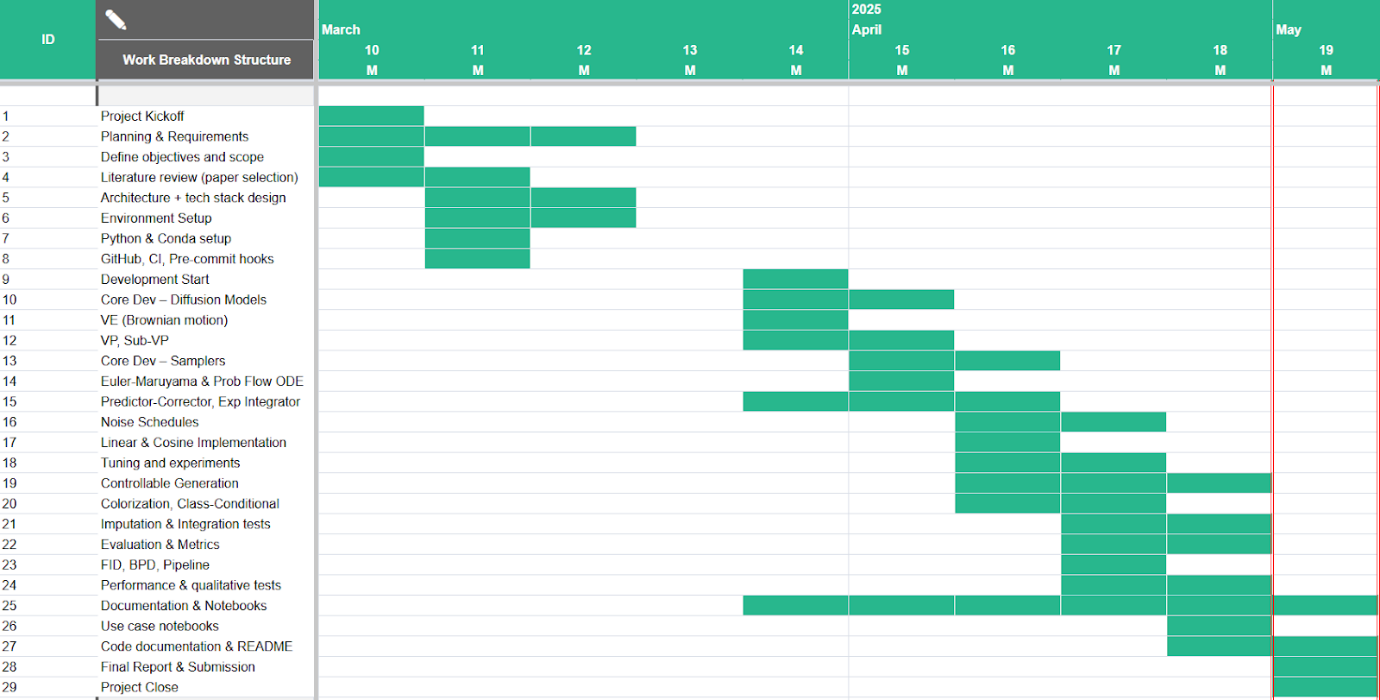
\includegraphics[width=0.8\textwidth]{img/page18_img1.png}
    \caption{Preview of the created Gantt Chart}
\end{figure}

\subsection{Project Requirements Analysis}
\subsubsection*{Functional Requirements}
\textbf{FR1 – Custom dataset loading:} The system must allow the user to input their own image datasets for training or generation tasks.
\begin{itemize}
    \item \textbf{FR1.1:} The system must accept datasets containing images in grayscale or RGB.
    \item \textbf{FR1.2:} All images must have the following dimensions: (number of images, channels, height, width).
    \item \textbf{FR1.3:} The system must validate that the images meet these conditions and reject those that do not.
\end{itemize}

\textbf{FR2 – Image preprocessing:} The system must apply consistent preprocessing to the input data.
\begin{itemize}
    \item \textbf{FR2.1:} Images must be normalized to the range [-1, 1].
    \item \textbf{FR2.2:} Images must be converted to PyTorch tensors and reorganized by channel if necessary.
    \item \textbf{FR2.3:} The system must transparently handle black-and-white or color images.
\end{itemize}

\textbf{FR3 – Diffusion model selection:} The system must allow selecting the type of diffusion process before training.
\begin{itemize}
    \item \textbf{FR3.1:} VP, Sub-VP, and VE variants must be available.
    \item \textbf{FR3.2:} VP and Sub-VP variants must be compatible with all implemented sampling methods.
    \item \textbf{FR3.3:} The VE variant cannot be used with the Exponential Integrator method.
    \item \textbf{FR3.4:} The system must warn the user if an invalid combination is chosen.
\end{itemize}

\textbf{FR4 – Noise scheduler configuration:} The system must allow selecting the noise schedule for the diffusion process.
\begin{itemize}
    \item \textbf{FR4.1:} At least linear and cosinusoidal schedules must be implemented.
    \item \textbf{FR4.2:} The choice of the schedule must be reflected in both the training and generation phases.
\end{itemize}

\textbf{FR5 – Score-based model training:} The system must provide a function that trains a score model based on supervised learning.
\begin{itemize}
    \item \textbf{FR5.1:} Training must log the loss function's evolution.
    \item \textbf{FR5.2:} The user must be able to adjust parameters such as epochs, batch size, and learning rate.
    \item \textbf{FR5.3:} There must be an explicit externally callable function, e.g., \texttt{train()}, encapsulating the entire process.
\end{itemize}

\textbf{FR6 – Image generation via sampling:} The system must offer a function to generate images from noise.
\begin{itemize}
    \item \textbf{FR6.1:} This function must implement the reverse diffusion process using a compatible integration method.
    \item \textbf{FR6.2:} The model must generate a batch of images and visualize the results in the environment.
    \item \textbf{FR6.3:} The function must be externally callable, e.g., \texttt{sample\_and\_plot()}, without needing to modify the codebase.
\end{itemize}

\textbf{FR7 – Sampling integrator selection:} The system must allow choosing the integration method to generate images.
\begin{itemize}
    \item \textbf{FR7.1:} Euler-Maruyama, Predictor-Corrector, Probability Flow ODE, and Exponential Integrator methods must be available.
    \item \textbf{FR7.2:} The selection must be user-configurable before initiating sampling.
\end{itemize}

\textbf{FR8 – Class-controlled generation:} The system must allow conditioning generation to specific classes when the dataset allows it.
\begin{itemize}
    \item \textbf{FR8.1:} The user must be able to specify a class (e.g., digits in MNIST).
    \item \textbf{FR8.2:} The system must verify that the model has been trained conditionally before proceeding.
\end{itemize}

\textbf{FR9 – Incomplete image imputation:} The system must support the reconstruction of partially observed images.
\begin{itemize}
    \item \textbf{FR9.1:} The user must be able to define a binary mask indicating the observed regions.
    \item \textbf{FR9.2:} The model must complete the missing regions via conditional sampling.
    \item \textbf{FR9.3:} Both the incomplete and the reconstructed image must be visualized.
\end{itemize}

\textbf{FR10 – Generated image quality evaluation:} The system must offer quantitative quality metrics.
\begin{itemize}
    \item \textbf{FR10.1:} Bits Per Dimension (BPD), Fréchet Inception Distance (FID), and Inception Score (IS) metrics must be implemented.
\end{itemize}

\textbf{FR11 – Saving and loading trained models:} The system must allow saving trained models and loading pre-existing ones.
\begin{itemize}
    \item \textbf{FR11.1:} The user must be able to specify the path to save the model.
    \item \textbf{FR11.2:} The system must save both the weights and the employed configuration.
    \item \textbf{FR11.3:} The user must be able to load a model from any valid path to perform sampling or evaluation.
\end{itemize}

\textbf{FR12 – Usage documentation and executable notebooks:} The system must include complete examples of the workflow.
\begin{itemize}
    \item \textbf{FR12.1:} Independent notebooks must be provided for training, generation, and evaluation tasks.
    \item \textbf{FR12.2:} The notebooks must include brief explanations and ordered cells, executable without manual intervention.
\end{itemize}

\textbf{FR13 – System testing:} The system must include tests to ensure the software's basic stability.
\begin{itemize}
    \item \textbf{FR13.1:} Simple unit tests must be implemented for key functions, such as data loading, normalization, or sampling.
    \item \textbf{FR13.2:} Tests must run automatically before training via a continuous integration environment (if enabled).
\end{itemize}

\textbf{FR14 – Minimal model performance validation:} The system must be able to train models that generate reasonable images on simple datasets.
\begin{itemize}
    \item \textbf{FR14.1:} On the MNIST dataset, the model must achieve acceptable visual quality in the generated samples.
    \item \textbf{FR14.2:} On the CIFAR-10 dataset, the model must generate blurry but visually recognizable structures.
\end{itemize}

\subsubsection*{Non-Functional Requirements}
\textbf{NFR1: Hardware Compatibility:} The system must run on both GPU and CPU, though GPU is recommended. Detection should be automatic. \\
\textbf{NFR2: Code Modularity:} The design must be modular, allowing independent replacement/configuration of components (diffusion model, sampler, noise planner, conditioning methods). \\
\textbf{NFR3: Ease of use via notebooks:} The system is controlled via well-organized Jupyter notebooks that execute sequentially without errors. \\
\textbf{NFR4: Reasonable runtime optimization:} Execution times must be acceptable. Training on small datasets shouldn't exceed an hour on GPU, and sampling should take seconds to minutes. \\
\textbf{NFR5: Automatic model management:} The system must auto-save trained models with descriptive names and allow reuse to prevent wasting resources. \\
\textbf{NFR6: Clear file and folder organization:} A clean folder structure must store trained models, generated results, and images with predictable paths and descriptive names. \\
\textbf{NFR7: Simple and explicit parameter configuration:} Key experiment parameters must be clearly stated at the beginning of scripts/notebooks.

\subsubsection*{Use Cases}
\textbf{Use Case 1: Training a model from scratch}\\
1. User provides a folder with images.\\
2. Indicates diffusion process (VP, Sub-VP, VE), noise planner, epochs, etc.\\
3. System trains the score model and saves it.

\textbf{Use Case 2: Image generation from noise}\\
1. User loads a trained model.\\
2. Chooses an integration method (e.g., Predictor-Corrector).\\
3. Calls \texttt{sample\_and\_plot()} with parameters. \\
4. System generates and displays images.

\textbf{Use Case 3: Model quality evaluation}\\
1. User loads a model and generates images.\\
2. System calculates BPD, FID, and IS.\\
3. User visualizes and compares the results.

\textbf{Use Case 4: Class-conditional generation}\\
1. User trains or loads a conditional model.\\
2. Calls the sampling function indicating the desired class.\\
3. System generates images conditioned to that label.

\textbf{Use Case 5: Incomplete image imputation}\\
1. User provides incomplete images and a binary mask.\\
2. System applies conditional sampling to fill in gaps.\\
3. Original, incomplete, and reconstructed images are shown.

\subsection{Design}
The project design was carefully structured to provide a modular, extensible, and reusable architecture centered on diffusion generative models. Organizationally, there is a clear separation between components: diffusion processes, numerical integrators (samplers), neural architecture (ScoreNet), training, image generation, YAML configuration, and conditioning systems (imputation or class generation). This allows experimenting with variants without altering the system's core.

The central \texttt{DiffusionExperiment} class acts as the main orchestrator, hiding internal logic from the end-user and allowing full system configuration via a dictionary or YAML file. The design supports interactive script usage, command-line usage, and real-project deployment. The network architecture is an adapted U-Net with Fourier embeddings for time and additional layers for conditioning.

Below is a preview of the system's class diagram; the complete version is in the Appendices.

\begin{figure}[H]
    \centering
    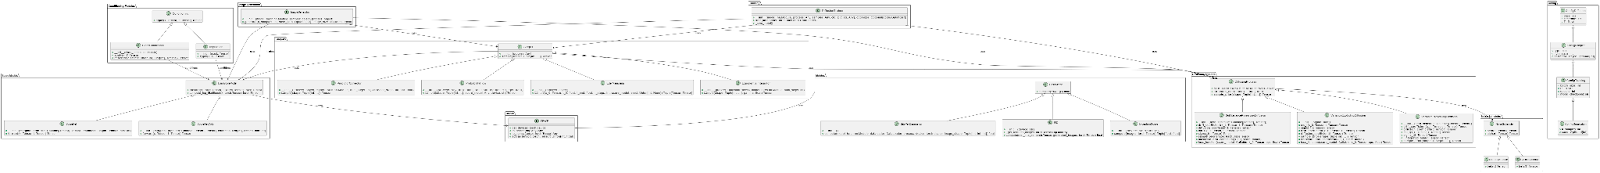
\includegraphics[width=0.8\textwidth]{img/page24_img1.png}
    \caption{Preview of the created Class Diagram}
\end{figure}

\subsection{Validation and Tests}
Unit and performance tests were executed for all components. Unit tests validate diffusion processes and samplers. A performance script measured execution times for 19 combinations of diffusion processes, samplers, and schedulers over 10 epochs. A CPU vs. GPU comparison confirmed efficiency improvements.

\subsection{Software Development and Quality Assurance}
Quality practices were applied: Git version control, PEP8 style guidelines, \texttt{black} for formatting, \texttt{flake8} for linting. Automated tests verify key components. Automatic documentation was generated using DeepWiki by CognitionLabs.

\subsection{Use License and Ethical Aspects}
\textbf{Use License:} For academic purposes. Code can be freely modified in this context.\\
\textbf{Ethical Aspects:} Restricted to simple public datasets (MNIST, CIFAR-10), without risk of generating inappropriate content or replicating discriminatory biases.

\section{Use Examples}
To demonstrate the functionality and capabilities of the system, several notebooks have been prepared to teach the use of the offered tools: training, image generation, evaluation, and advanced applications. Each of them attempts to expose the handling of the model and facilitate its understanding.

In the first notebook, model training is performed using only the digit 3 images from MNIST. Here, the three available types of diffusion processes are explained and implemented: VE (Variance Exploding), VP (Variance Preserving), and Sub-VP. The user is shown how to use the different training configurations, including the noise schedules (linear or cosine). The models generated in this step are saved in a \texttt{checkpoints} folder and reused in the following notebooks.

The second notebook focuses on the sampling and visualization process. Using the models trained in notebook 01, the different image generation algorithms are tested: Euler-Maruyama, Predictor-Corrector, Probability Flow ODE, and Exponential Integrator. The effects of changing certain sampling hyperparameters in each sampler are explained, as well as how to modify the number of sampler steps. In this demo, the results of all samplers combined with the 3 trained diffusion models are visualized.

In the third notebook, both training and sampling explained in previous demos are applied, but this time on a color dataset. The 'boat' class (8) of the CIFAR-10 dataset is used. This case serves to verify that the system can generalize and adapt to color image generation, showing that there are barely any differences compared to black-and-white generation.

The fourth notebook is dedicated to evaluating model performance. It is a very basic notebook that takes a previously trained model and simply displays metrics such as BPD, FID (Fréchet Inception Distance), and IS (Inception Score), which measure the quality of the generated images. A brief explanation is given for each metric so the user understands how they work.

Finally, the fifth notebook (05) deals with the use of the model for conditioning and image imputation. For conditioning, images are generated from prior or partial information, such as a class or a visible section. In the imputation part, it demonstrates how the model is capable of completing images that have erased or missing parts, generating content coherent with the rest of the image. This demo is performed with different MNIST digits and shows how to train the models for these tasks. Following this, the results are visualized and the demo ends.

\section{Conclusion}
This work has shown how diffusion models can be used effectively to generate controlled images and manipulate visual data accurately. By training a U-Net-based network from scratch, along with information about time and the desired class, it was even possible to guide the generative process to produce images that clearly respond to an indicated category. For this, a technique known as classifier-free guidance was applied, which adjusts the outcome during generation using gradients from the class embedding.

The results show that the model is capable of generating coherent and recognizable images from noise, which demonstrates that it has learned useful relationships between classes and visual forms. It has also been seen that adjusting the guidance intensity according to the time step improves the balance between visual precision and sample variety.

However, working with limited computational resources has imposed some restrictions. For example, it was necessary to reduce the model size and the number of training steps, which affects the final quality of the images compared to larger systems. Despite these limitations, the results obtained are very promising: they show that even with modest means, diffusion models can generate realistic and controlled images, and pave the way for applications such as partial editing, image reconstruction, or visual content creation from structured descriptions.

\begin{thebibliography}{99}
\bibitem{dhariwal2021} Dhariwal, P., \& Nichol, A. (2021). Diffusion models beat GANs on image synthesis. arXiv. \url{https://arxiv.org/abs/2105.0523}
\bibitem{ho2020} Ho, J., Jain, A., \& Abbeel, P. (2020). Denoising diffusion probabilistic models. arXiv. \url{https://arxiv.org/abs/2006.11239}
\bibitem{zhao} Zhao, W., Bai, L., Rao, Y., Zhou, J., \& Lu, J. UniPC: A unified predictor-corrector framework for fast sampling of diffusion models. Tsinghua University. \url{https://arxiv.org/pdf/2302.04867}
\bibitem{zhang} Zhang, Q., \& Chen, Y. Fast sampling of diffusion models with exponential integrator. Georgia Institute of Technology. \url{https://arxiv.org/pdf/2204.13902}
\bibitem{song2021} Song, Y., Sohl-Dickstein, J., Kingma, D. P., Kumar, A., Ermon, S., \& Poole, B. (2021). Score-based generative modeling through stochastic differential equations. ICLR. \url{https://openreview.net/forum?id=PxTIG12RRHS}
\end{thebibliography}

\appendix
\section{Sample Images}
Below are some of the images obtained throughout the project as a sample or demo of its functionality.

\begin{figure}[H]
    \centering
    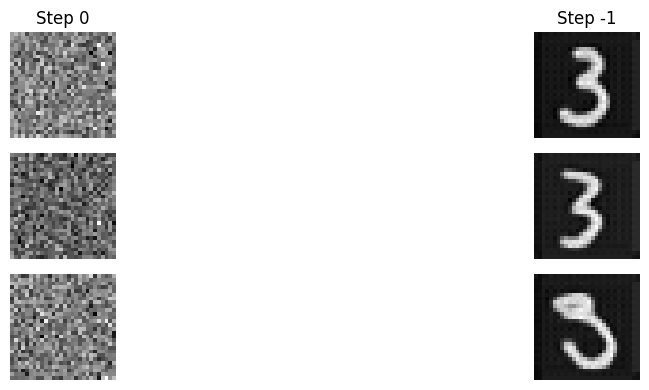
\includegraphics[width=0.5\textwidth]{img/page44_img1.png}
    \caption{Digit 3 MNIST with VP (cosine) and Probability Flow ODE}
\end{figure}

\begin{figure}[H]
    \centering
    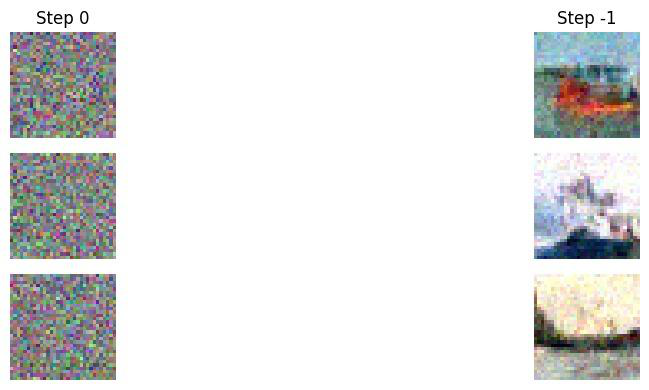
\includegraphics[width=0.5\textwidth]{img/page48_img2.png}
    \caption{Boats CIFAR-10 with VE and Predictor Corrector}
\end{figure}

\begin{figure}[H]
    \centering
    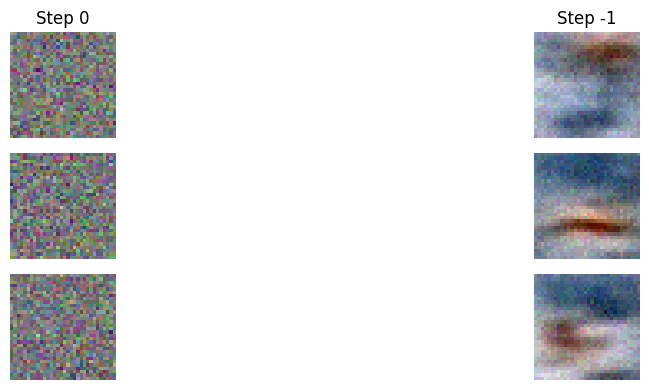
\includegraphics[width=0.5\textwidth]{img/page51_img1.png}
    \caption{Boats with VP and Predictor Corrector}
\end{figure}

\begin{figure}[H]
    \centering
    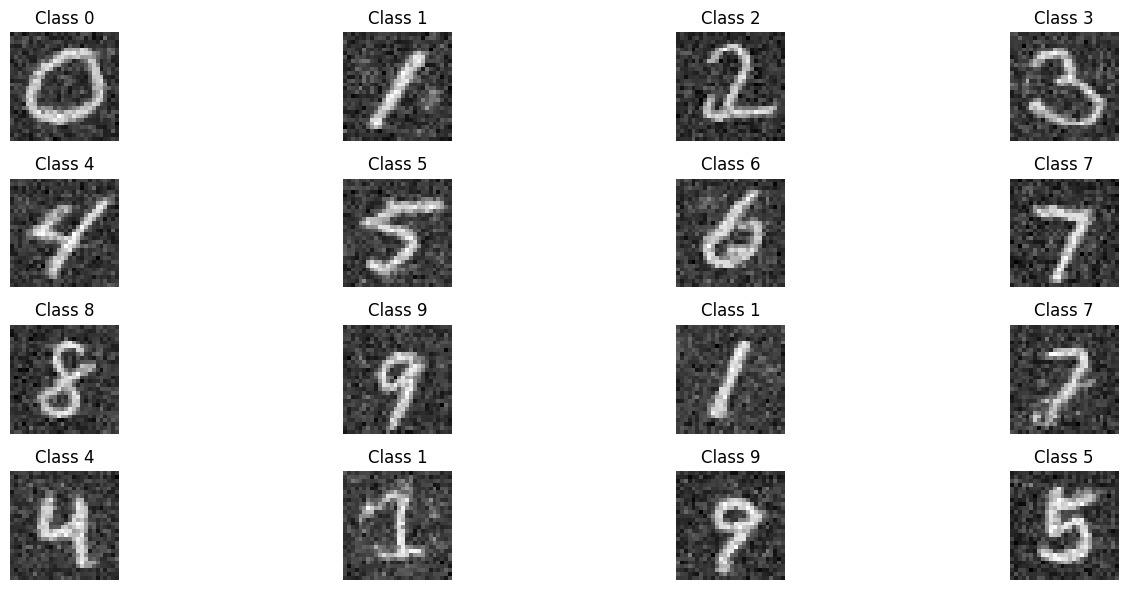
\includegraphics[width=0.5\textwidth]{img/page51_img2.png}
    \caption{Conditional generation by class}
\end{figure}

\begin{figure}[H]
    \centering
    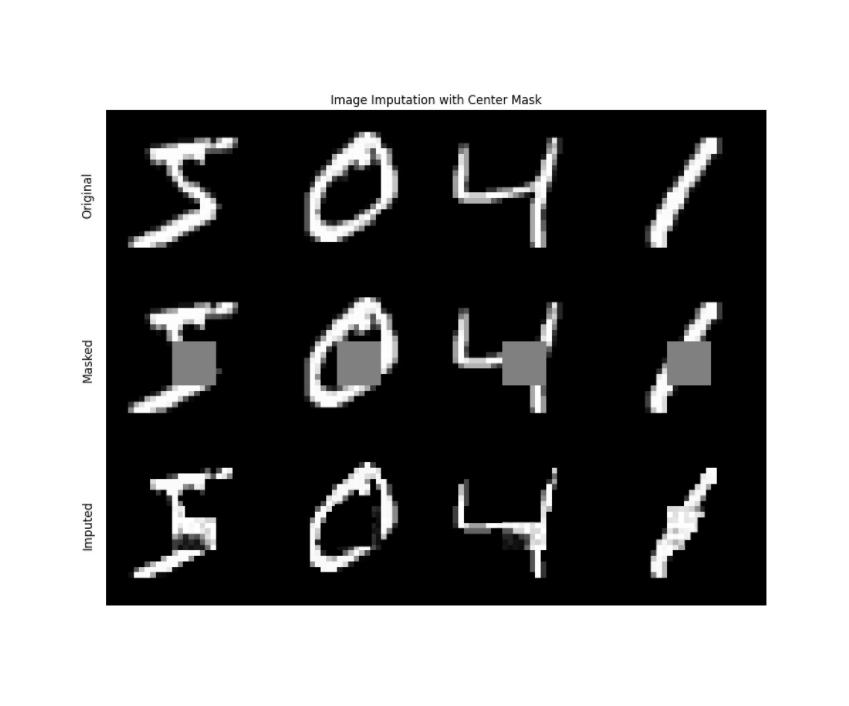
\includegraphics[width=0.5\textwidth]{img/page52_img1.png}
    \caption{Imputation of masks/missing regions}
\end{figure}

\end{document}
